%%%%%%%%%%%%%%%%%%%%%%%%%%%%%%%%%%%%%%%%%
% Jacobs Portrait Poster
% LaTeX Template
% Version 1.0 (31/08/2015)
% (Based on Version 1.0 (29/03/13) of the landscape template
%
% Created by:
% Computational Physics and Biophysics Group, Jacobs University
% https://teamwork.jacobs-university.de:8443/confluence/display/CoPandBiG/LaTeX+Poster
%
% Further modified by:
% Nathaniel Johnston (nathaniel@njohnston.ca)
%
% Portrait version by:
% John Hammersley
%
% The landscape version of this template was downloaded from:
% http://www.LaTeXTemplates.com
%
% License:
% CC BY-NC-SA 3.0 (http://creativecommons.org/licenses/by-nc-sa/3.0/)
%
%%%%%%%%%%%%%%%%%%%%%%%%%%%%%%%%%%%%%%%%%

%----------------------------------------------------------------------------------------
%    PACKAGES AND OTHER DOCUMENT CONFIGURATIONS
%----------------------------------------------------------------------------------------

\documentclass[final]{beamer}

\usepackage[size=a1, orientation=portrait, scale=0.74]{beamerposter} % Use the beamerposter package for laying out the poster

\usetheme{confposter} % Use the confposter theme supplied with this template
\usepackage{tikz}
\usetikzlibrary{calc,arrows.meta,positioning,shapes.geometric,fit,backgrounds}

\usepackage{amsmath,amssymb,amsfonts}
\usepackage{textcomp}
\usepackage{xcolor}

% NOTE: To change colors, change lines 26-29 in beamerthemeconfposter.sty
\setbeamercolor{block title}{fg=headerTitle,bg=white} % Colors of the block titles
\setbeamercolor{block body}{fg=black,bg=white} % Colors of the body of blocks
\setbeamercolor{block alerted title}{fg=alertColor,bg=headerOuter!90} % Colors of the highlighted block titles

%-----------------------------------------------------------
% Define the column widths and overall poster size
% To set effective sepwid, onecolwid and twocolwid values, first choose how many columns you want and how much separation you want between columns
% In this template, the separation width chosen is 0.024 of the paper width and a 4-column layout
% onecolwid should therefore be (1-(# of columns+1)*sepwid)/# of columns e.g. (1-(4+1)*0.024)/4 = 0.22
% Set twocolwid to be (2*onecolwid)+sepwid = 0.464
% Set threecolwid to be (3*onecolwid)+2*sepwid = 0.708

\newlength{\sepwid}
\newlength{\colwid}
\setlength{\paperwidth}{23.4in} % A1 width: 23.4in
\setlength{\paperheight}{33.1in} % A1 height: 33.1in
\setlength{\sepwid}{0.024\paperwidth} % Separation width (white space) between columns
\setlength{\colwid}{0.464\paperwidth} % Width of one column
\setlength{\topmargin}{-0.5in} % Reduce the top margin size
%-----------------------------------------------------------

\usepackage{graphicx}  % Required for including images

\usepackage{booktabs} % Top and bottom rules for tables
\usepackage{tabularx} % Tables that stretch to fill the available width

% Colors used inside the TikZ diagrams (kept independent of the theme's
% internal color names so the diagrams render even if the theme palette
% changes).
\definecolor{stateColor}{RGB}{225,238,252}
\definecolor{fnColor}{RGB}{255,236,210}
\definecolor{boxColor}{RGB}{240,240,240}
\definecolor{arrowColor}{RGB}{60,60,60}

% Fixed absolute point sizes for TikZ diagram labels. The poster's \small /
% \diagsmallfont / \scriptsize are rescaled by beamerposter's font-scale
% machinery (tied to the "scale" option above) and can end up far larger
% than intended, which silently forces TikZ nodes to expand past their
% "minimum width" to fit the text -- deliberately NOT using those commands
% inside diagrams avoids that.
\newcommand{\diagfont}{\fontsize{15}{17}\selectfont}
\newcommand{\diagsmallfont}{\fontsize{11}{13}\selectfont}

%----------------------------------------------------------------------------------------
%    TITLE SECTION
%----------------------------------------------------------------------------------------

\title{Data Flyway \\ \Large In-flight Analysis for Object-centric HPC Data Management} % Poster title

\author{Noah Lewis, Abdullah Al Raqibul Islam, Suren Byna} % Author(s)

\institute{Integration Team} % Institution(s)

%----------------------------------------------------------------------------------------

\begin{document}

\addtobeamertemplate{block end}{}{\vspace*{1ex}} % White space under blocks
\addtobeamertemplate{block alerted end}{}{\vspace*{2ex}} % White space under highlighted (alert) blocks

\setlength{\belowcaptionskip}{2ex} % White space under figures
\setlength\belowdisplayshortskip{2ex} % White space under equations

\begin{frame}[t] % The whole poster is enclosed in one beamer frame

\begin{columns}[t] % The whole poster will consist of two columns.

\begin{column}{\sepwid}\end{column} % Empty spacer column

\begin{column}{\colwid} % The first column

%----------------------------------------------------------------------------------------
%    MOTIVATION
%----------------------------------------------------------------------------------------

\begin{alertblock}{Motivation}
  SAGEST workflows routinely need \textbf{derived} data products. A HashBrick
  CFD solver used in SAGEST workloads, for example, persists per-brick
  conserved fields ($\rho,\rho u,\rho v,\rho w,\rho e$) every timestep. The diagnostics
  engineers actually want, velocity magnitude, vorticity, pressure, require a
  separate manual read-compute-write \textbf{outside} PDC today
  (Figure~\ref{fig:sagest}). PDC already transforms a \textbf{single} object
  transparently on I/O (compression, encryption), but has no way to produce a
  derived object from \textbf{multiple} inputs. We close that gap with a new
  PDC \textbf{analysis} extension: multi-input, multi-output derived
  computation built directly into the I/O path.

  \begin{center}
  \begin{figure}
    \begin{tikzpicture}[
        state/.style={draw, rounded corners, fill=stateColor, minimum width=3.3cm, minimum height=1.3cm, align=center, font=\diagfont},
        gapstate/.style={draw, dashed, rounded corners, fill=white, minimum width=3.3cm, minimum height=1.3cm, align=center, font=\diagfont},
        fn/.style={draw, fill=fnColor, minimum width=2.6cm, minimum height=1cm, align=center, font=\diagfont},
        arr/.style={-{Latex[length=2.5mm]}, thick, arrowColor},
        gaparr/.style={-{Latex[length=2.5mm]}, thick, dashed, arrowColor},
        >=Latex, node distance=1.9cm
      ]
      \node[fn] (sim) {HashBrick\\ \diagsmallfont CFD solver};
      \node[state, right=of sim] (fields) {$\rho,\rho u,\rho v,\rho w,\rho e$ \\ \diagsmallfont persisted every timestep};
      \node[gapstate, right=3.8cm of fields] (derived) {$|u|$, vorticity, pressure \\ \diagsmallfont needed for analysis};

      \draw[arr] (sim) -- node[above, font=\diagsmallfont]{write} (fields);
      \draw[gaparr] (fields) -- node[above, font=\diagsmallfont, align=center]{today: manual\\ read-compute-write} (derived);
    \end{tikzpicture}
    \caption{\diagsmallfont The dashed step is where PDC analysis plugs in:
    computing derived diagnostics directly in the I/O path instead of a
    separate pass.}
    \label{fig:sagest}
  \end{figure}
  \end{center}
\end{alertblock}

%----------------------------------------------------------------------------------------
%    BACKGROUND: TRANSFORMATION FRAMEWORK
%----------------------------------------------------------------------------------------
\begin{block}{Background: PDC's Transformation Framework}
PDC's transformation framework already moves \textbf{one} object between named
states (e.g.\ \texttt{raw}$\to$\texttt{compressed}) transparently on write and
read, as a single-input, single-output pipeline.

\begin{center}
  \begin{figure}
    \begin{tikzpicture}[
        state/.style={draw, rounded corners, fill=stateColor, minimum width=2.6cm, minimum height=1cm, align=center, font=\diagfont},
        fn/.style={draw, fill=fnColor, minimum width=2.6cm, minimum height=1cm, align=center, font=\diagfont},
        arr/.style={-{Latex[length=2.5mm]}, thick, arrowColor},
        >=Latex
      ]
      \node[state] (raw) {raw \\ \diagsmallfont (client)};
      \node[fn, right=1.6cm of raw] (tf) {transform};
      \node[state, right=1.6cm of tf] (comp) {compressed \\ \diagsmallfont (storage)};

      \draw[arr] (raw) -- node[above, font=\diagsmallfont]{write} (tf);
      \draw[arr] (tf) -- node[above, font=\diagsmallfont]{store} (comp);
      \draw[arr] (comp.south) .. controls +(0,-1.1) and +(0,-1.1) .. node[below, font=\diagsmallfont]{read: invert transparently} (raw.south);
    \end{tikzpicture}
    \caption{\diagsmallfont The inverse transform on read is fully transparent: no explicit ``run'' call.}
  \end{figure}
\end{center}
\end{block}

%----------------------------------------------------------------------------------------
%    ANALYSIS FRAMEWORK
%----------------------------------------------------------------------------------------
\begin{block}{Generalizing to Multi-Object Analysis Graphs}
Our extension allows \textbf{multiple} named inputs and outputs, defined in a
JSON graph attached to PDC objects at runtime; a function node can fan-in from
several inputs and fan-out to several outputs.

\begin{center}
  \begin{figure}
    \begin{tikzpicture}[
        state/.style={draw, rounded corners, fill=stateColor, minimum width=2.5cm, minimum height=0.9cm, align=center, font=\diagfont},
        fn/.style={draw, fill=fnColor, minimum width=2.6cm, minimum height=0.9cm, align=center, font=\diagfont},
        arr/.style={-{Latex[length=2.5mm]}, thick, arrowColor},
        >=Latex, node distance=1.1cm and 1.6cm
      ]
      \node[state] (temp) {temp\_in \\ \diagsmallfont transient};
      \node[state, below=of temp] (pres) {pressure\_in \\ \diagsmallfont transient};
      \coordinate (midin) at ($(temp)!0.5!(pres)$);
      \node[fn, right=1.6cm of midin] (merge) {merge\_fields};
      \node[state, right=1.6cm of merge] (merged) {merged \\ \diagsmallfont transient};
      \node[fn, right=1.6cm of merged] (reduce) {reduce\_stats};
      \node[state, above right=0.3cm and 1.6cm of reduce] (mean) {stats\_mean \\ \diagsmallfont persistent};
      \node[state, below right=0.3cm and 1.6cm of reduce] (debug) {stats\_debug \\ \diagsmallfont persistent};

      \draw[arr] (temp) -- (merge);
      \draw[arr] (pres) -- (merge);
      \draw[arr] (merge) -- (merged);
      \draw[arr] (merged) -- (reduce);
      \draw[arr] (reduce) -- (mean);
      \draw[arr] (reduce) -- (debug);
    \end{tikzpicture}
    \caption{\diagsmallfont Two inputs feed a fan-in function; its transient output feeds a
    fan-out function producing two independently-readable outputs.}
  \end{figure}
\end{center}

Attaching a state marks it as a source or a sink; reading an unmaterialized
output transparently triggers only the computation still needed.
\end{block}

%----------------------------------------------------------------------------------------
%    STATUS
%----------------------------------------------------------------------------------------
\begin{block}{Current Status}
The core analysis framework is implemented and working end to end:
\begin{itemize}
  \item Graphs are defined in JSON and attached via the client API.
  \item Both eager and lazy execution are supported (see right), computing
        only what a given output still needs.
  \item Composes with the transformation framework: an analysis output can
        itself be compressed or transformed.
  \item \texttt{vector\_magnitude} passes end-to-end tests.
\end{itemize}
\end{block}

%----------------------------------------------------------------------------------------
%    IMPLEMENTATION NOTES
%----------------------------------------------------------------------------------------
\begin{block}{Implementation Notes}
Attachment reuses machinery the transformation framework already has, instead
of adding a new RPC path:
\begin{itemize}
  \item A graph's attachments are assembled once on the client and embedded
        in the next write request, the same way the transformation framework
        already extends its write requests.
  \item Regions partition statically: a rank's disjoint region routes to the
        matching server automatically, with no client-side tracking of
        server ranks.
  \item The server executes the graph against only the states a read
        actually needs, not the whole graph unconditionally.
\end{itemize}

\begin{center}
  \begin{figure}
    \begin{tikzpicture}[
        state/.style={draw, rounded corners, fill=stateColor, minimum width=2.6cm, minimum height=1.1cm, align=center, font=\diagfont},
        fn/.style={draw, fill=fnColor, minimum width=3.6cm, minimum height=1.1cm, align=center, font=\diagfont},
        arr/.style={-{Latex[length=2.5mm]}, thick, arrowColor},
        >=Latex, node distance=1.4cm
      ]
      \node[state] (client) {client \\ \diagsmallfont write(vx,vy,vz)};
      \node[fn, right=of client] (rpc) {write request \\ \diagsmallfont embeds attachment info};
      \node[state, right=of rpc] (server) {server \\ \diagsmallfont materializes reachable outputs};

      \draw[arr] (client) -- (rpc);
      \draw[arr] (rpc) -- (server);
    \end{tikzpicture}
    \caption{\diagsmallfont Graph attachment is embedded in the existing write
    request: no separate attach round trip, no client-side server-rank
    bookkeeping.}
  \end{figure}
\end{center}
\end{block}

\end{column} % End of left column

%----------------------------------------------------------------------------------------
\begin{column}{\sepwid}\end{column} % Empty spacer column

\begin{column}{\colwid} % Beginning of second column

%----------------------------------------------------------------------------------------
%    ANALYSIS TASK GRAPHS
%----------------------------------------------------------------------------------------
\begin{block}{Analysis Task Graphs}

Two implemented graphs show the model in practice.

\begin{center}
  \begin{figure}
    \begin{tikzpicture}[
        state/.style={draw, rounded corners, fill=stateColor, minimum width=2.3cm, minimum height=0.85cm, align=center, font=\diagfont},
        fn/.style={draw, fill=fnColor, minimum width=3.1cm, minimum height=0.85cm, align=center, font=\diagfont},
        arr/.style={-{Latex[length=2.5mm]}, thick, arrowColor},
        >=Latex, node distance=0.5cm and 2.2cm
      ]
      \node[state] (vx) {vx \\ \diagsmallfont persistent};
      \node[state, below=of vx] (vy) {vy \\ \diagsmallfont persistent};
      \node[state, below=of vy] (vz) {vz \\ \diagsmallfont persistent};
      \node[fn, right=2.2cm of vy] (fn) {vector\_magnitude \\ \diagsmallfont builtin, CPU};
      \node[state, right=2.2cm of fn] (mag) {magnitude \\ \diagsmallfont persistent};

      \draw[arr] (vx) -- (fn);
      \draw[arr] (vy) -- (fn);
      \draw[arr] (vz) -- (fn);
      \draw[arr] (fn) -- (mag);
    \end{tikzpicture}
    \caption{\diagsmallfont \texttt{vector\_magnitude}: magnitude directly from
    three persistent vector-component inputs.}
  \end{figure}
\end{center}

\begin{center}
  \begin{figure}
    \begin{tikzpicture}[
        state/.style={draw, rounded corners, fill=stateColor, minimum width=2.1cm, minimum height=0.8cm, align=center, font=\diagfont},
        fn/.style={draw, fill=fnColor, minimum width=2.5cm, minimum height=0.8cm, align=center, font=\diagfont},
        arr/.style={-{Latex[length=2.5mm]}, thick, arrowColor},
        >=Latex, node distance=0.4cm and 1.8cm
      ]
      \node[state] (u) {u \\ \diagsmallfont persistent};
      \node[state, below=of u] (v) {v \\ \diagsmallfont persistent};
      \node[state, below=of v] (w) {w \\ \diagsmallfont persistent};
      \node[fn, right=1.8cm of v] (curl) {curl \\ \diagsmallfont external, CPU};
      \node[state, right=1.8cm of curl, yshift=0.85cm] (cx) {curl\_x \\ \diagsmallfont transient};
      \node[state, right=1.8cm of curl] (cy) {curl\_y \\ \diagsmallfont transient};
      \node[state, right=1.8cm of curl, yshift=-0.85cm] (cz) {curl\_z \\ \diagsmallfont transient};
      \node[fn, right=1.8cm of cy] (vm) {vector\_magnitude \\ \diagsmallfont builtin, CPU};
      \node[state, right=1.8cm of vm] (vmag) {vorticity\_magnitude \\ \diagsmallfont persistent};

      \draw[arr] (u) -- (curl);
      \draw[arr] (v) -- (curl);
      \draw[arr] (w) -- (curl);
      \draw[arr] (curl) -- (cx);
      \draw[arr] (curl) -- (cy);
      \draw[arr] (curl) -- (cz);
      \draw[arr] (cx) -- (vm);
      \draw[arr] (cy) -- (vm);
      \draw[arr] (cz) -- (vm);
      \draw[arr] (vm) -- (vmag);
    \end{tikzpicture}
    \caption{\diagsmallfont \texttt{curl\_vorticity\_magnitude}: an external
    \texttt{curl} composed with the builtin \texttt{vector\_magnitude}, computing
    vorticity magnitude from a velocity field \texttt{(u,v,w)}.}
  \end{figure}
\end{center}

\textbf{Composes with transformations.} An analysis output can itself be
compressed or transformed; that attachment is registered when the analysis
graph is attached.
\end{block}

%----------------------------------------------------------------------------------------
%    EAGER VS LAZY
%----------------------------------------------------------------------------------------
\begin{block}{Eager vs.\ Lazy Analysis Execution}
A graph's outputs can be materialized at two different times, and the analysis
framework supports both:

\begin{itemize}
  \item \textbf{Lazy (read-triggered).} Computed on first read; never touched
        if never read, but that first read pays the full compute cost.
  \item \textbf{Eager (write-triggered).} Computed proactively once inputs are
        ready, so a read just returns already-materialized data.
\end{itemize}

\vspace{0.15cm}
\renewcommand{\arraystretch}{1.15}
\begin{tabularx}{\linewidth}{@{} >{\raggedright\arraybackslash}p{0.16\linewidth} | >{\raggedright\arraybackslash}X | >{\raggedright\arraybackslash}X @{}}
    \toprule
     & \textbf{Lazy (on read)} & \textbf{Eager (on write)} \\
    \midrule
    Unread outputs & never computed & may compute anyway if reachable \\
    Read latency & pays compute cost first read & fast, already materialized \\
    Write latency & unaffected & extra computation per write \\
    \bottomrule
\end{tabularx}
\vspace{0.1cm}

One graph definition serves both patterns automatically, with no client-side
strategy choice.
\end{block}

%----------------------------------------------------------------------------------------
%    RESULTS
%----------------------------------------------------------------------------------------
\begin{block}{Results: Benefit at Scale}
We compared three ways to produce a derived object (magnitude from three
vector components) across 1 to 8 matched client/server ranks, 1\,GB of data per
rank:

\begin{center}
  \begin{figure}
    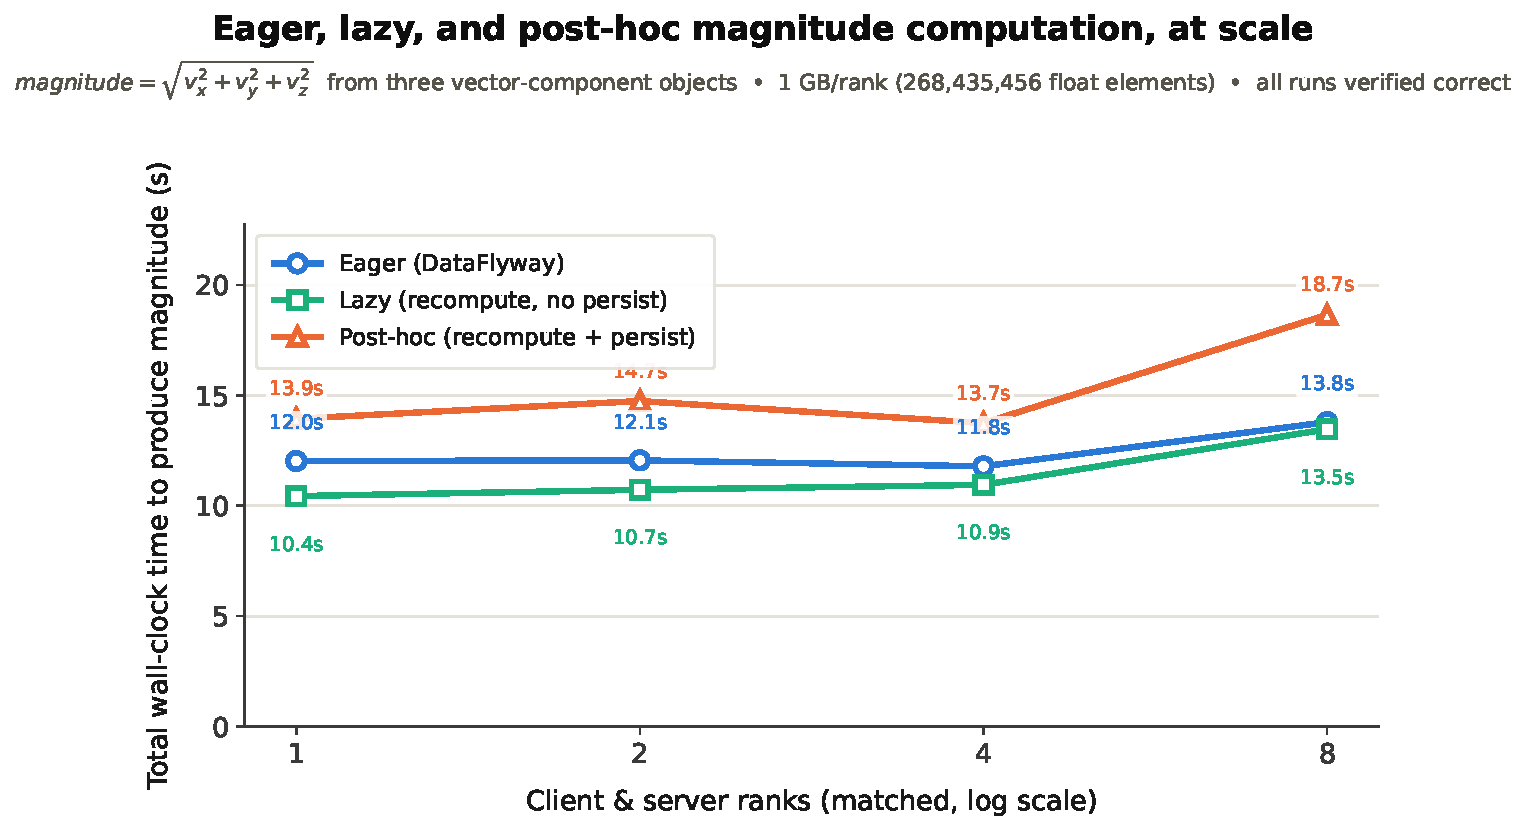
\includegraphics[width=0.92\linewidth]{pdc_scaling_plot.pdf}
  \end{figure}
\end{center}
\vspace{-0.3cm}

\textbf{Lazy} and \textbf{eager} both consistently beat \textbf{post-hoc}
(read components back, compute, write the result manually outside PDC).
Post-hoc pays an extra write every time; lazy and eager avoid it by either
never persisting or persisting as a side effect of work already happening
in the I/O path.
\end{block}

%----------------------------------------------------------------------------------------
%    FUTURE WORK
%----------------------------------------------------------------------------------------
\begin{block}{Future Work}
\begin{itemize}
  \item Validate these results at true HPC scale: more nodes, larger data,
        production SAGEST workloads.
  \item Add more builtin functions guided by SAGEST use cases.
  \item Explore GPU scheduling for analysis functions.
\end{itemize}
\end{block}

\end{column} % End of the second column

\begin{column}{\sepwid}\end{column} % Empty spacer column
%----------------------------------------------------------------------------------------

\end{columns} % End of poster

\end{frame} % End of the enclosing frame

\end{document}
